\documentclass{standalone}
\usepackage{tikz}
\usepackage{pgfplots}

\pgfplotsset{width=20cm,compat=1.5}

\begin{document}

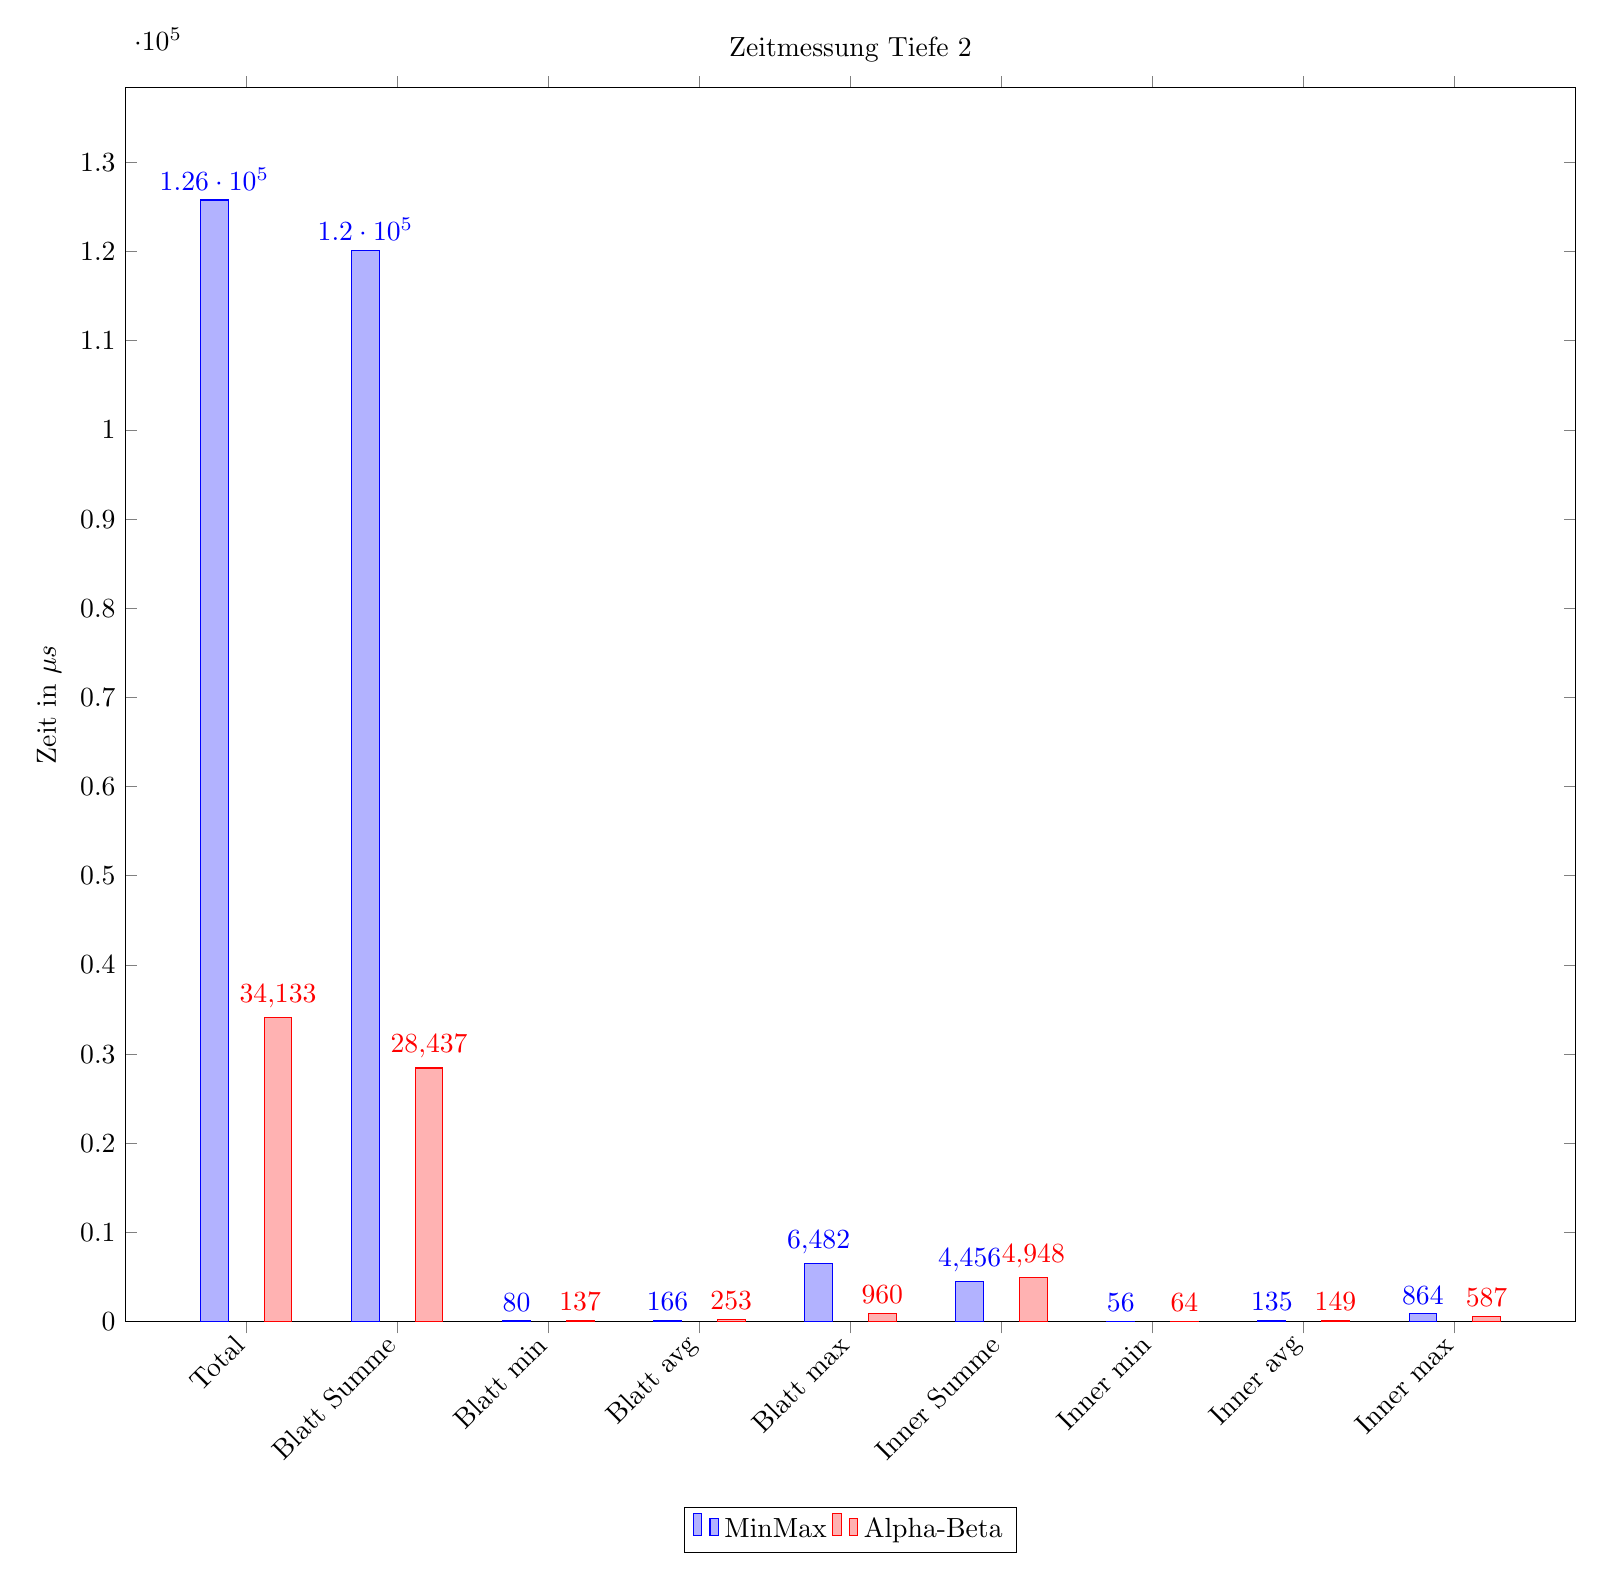
\begin{tikzpicture}
  \begin{axis}[
    title=Zeitmessung Tiefe 2,
    ybar=13pt,
    legend style={at={(0.5,-0.15)},
    anchor=north,
    legend columns=-1},
    ylabel={Zeit in $\mu s$},
    ymin = 0,
    symbolic x coords={
      Total,
      Blatt Summe,
      Blatt min,
      Blatt avg,
      Blatt max,
      Inner Summe,
      Inner min,
      Inner avg,
      Inner max
    },
    xtick=data,
    nodes near coords,
    nodes near coords align={vertical},
    x tick label style={rotate=45,anchor=east}
  ]
    \addplot coordinates{
      (Total,       125780)
      (Blatt Summe, 120120)
      (Blatt min,       80)
      (Blatt avg,      166)
      (Blatt max,     6482)
      (Inner Summe,   4456)
      (Inner min,       56)
      (Inner avg,      135)
      (Inner max,      864)
    };
    \addplot coordinates{
      (Total,       34133)
      (Blatt Summe, 28437)
      (Blatt min,     137)
      (Blatt avg,     253)
      (Blatt max,     960)
      (Inner Summe,  4948)
      (Inner min,      64)
      (Inner avg,     149)
      (Inner max,     587)
    };
    \legend{
      MinMax,
      Alpha-Beta
    }
  \end{axis}
\end{tikzpicture}


\end{document}